%\begin{figure}[t]
%	\centering
%			\centering
%			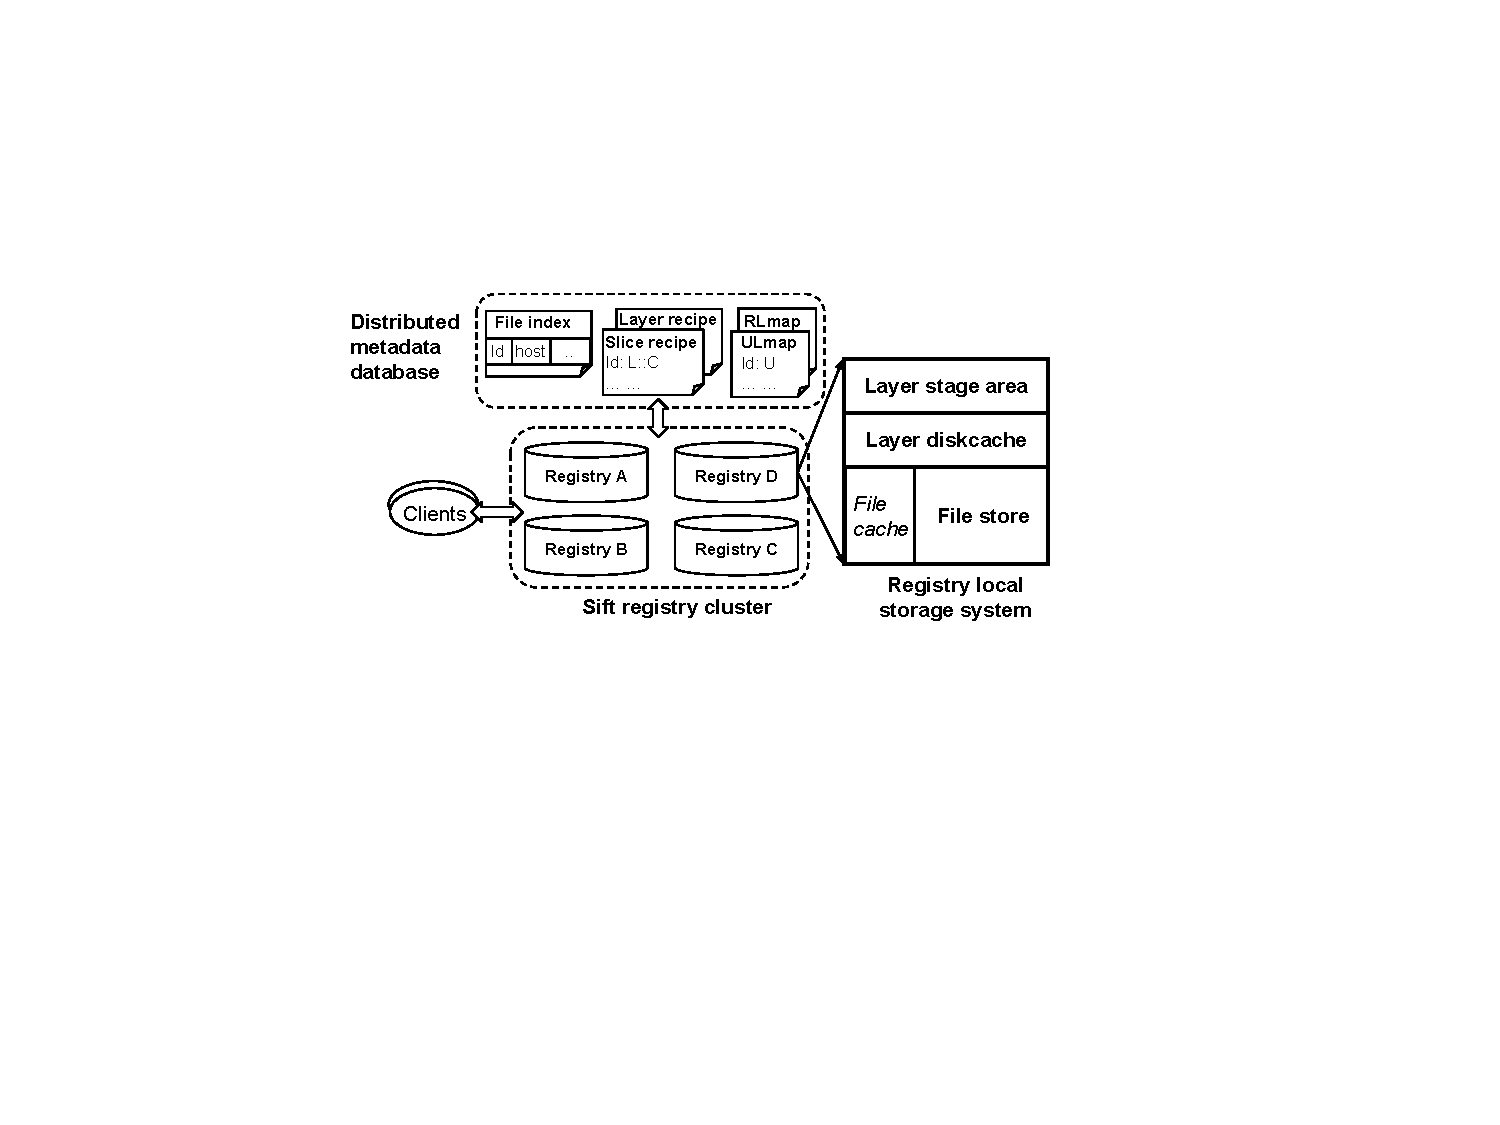
\includegraphics[width=0.40\textwidth]{graphs/sys-architecture.pdf}
%			\caption{Architecture of \sysname.}
%		\label{fig:sys-overview}
%\end{figure}

%\begin{figure}[t]
%	\centering
%	\centering
%	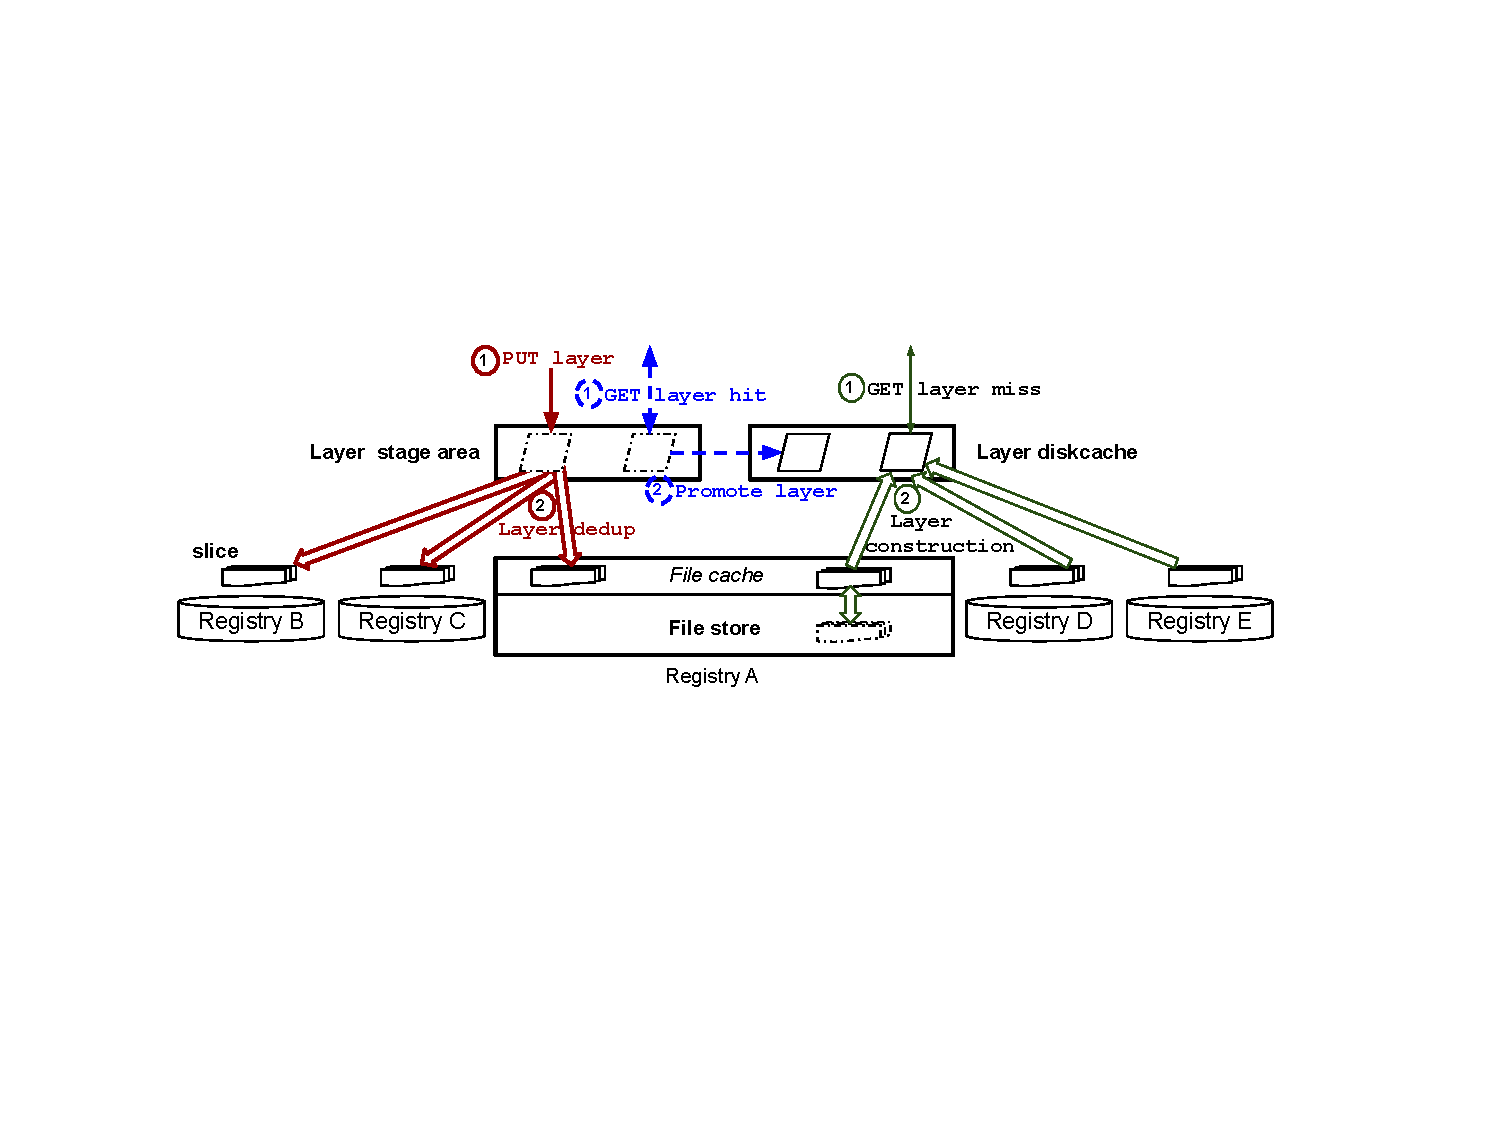
\includegraphics[width=0.5\textwidth]{graphs/sift-diskcache.pdf}
%	\caption{Sift cache.}
%	\label{fig:construct}
%\end{figure}

\begin{figure}[!t]
	\centering
	\subfigure[\sysname storage system]{
		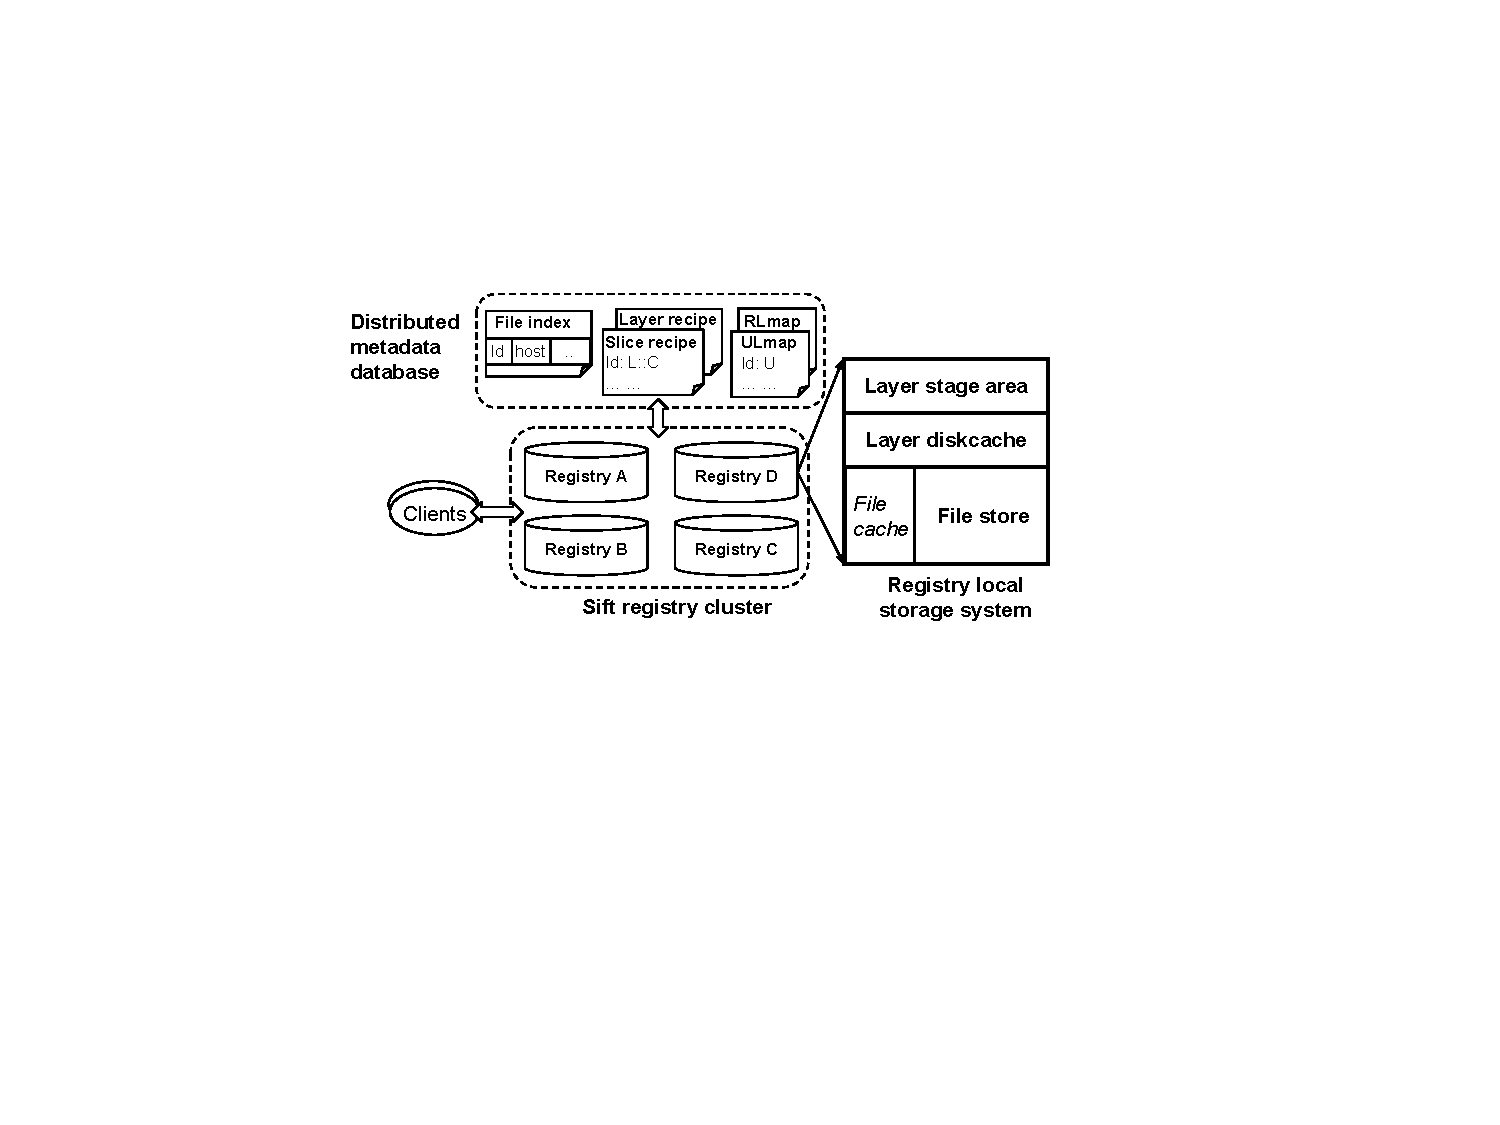
\includegraphics[width=0.35\textwidth]{graphs/sys-architecture.pdf}
		\label{fig:sift}
	}
	\subfigure[\sysname vs. original registry \LR{We should remove the original registry in that
	figure as it has already been discussed in the background}]{
		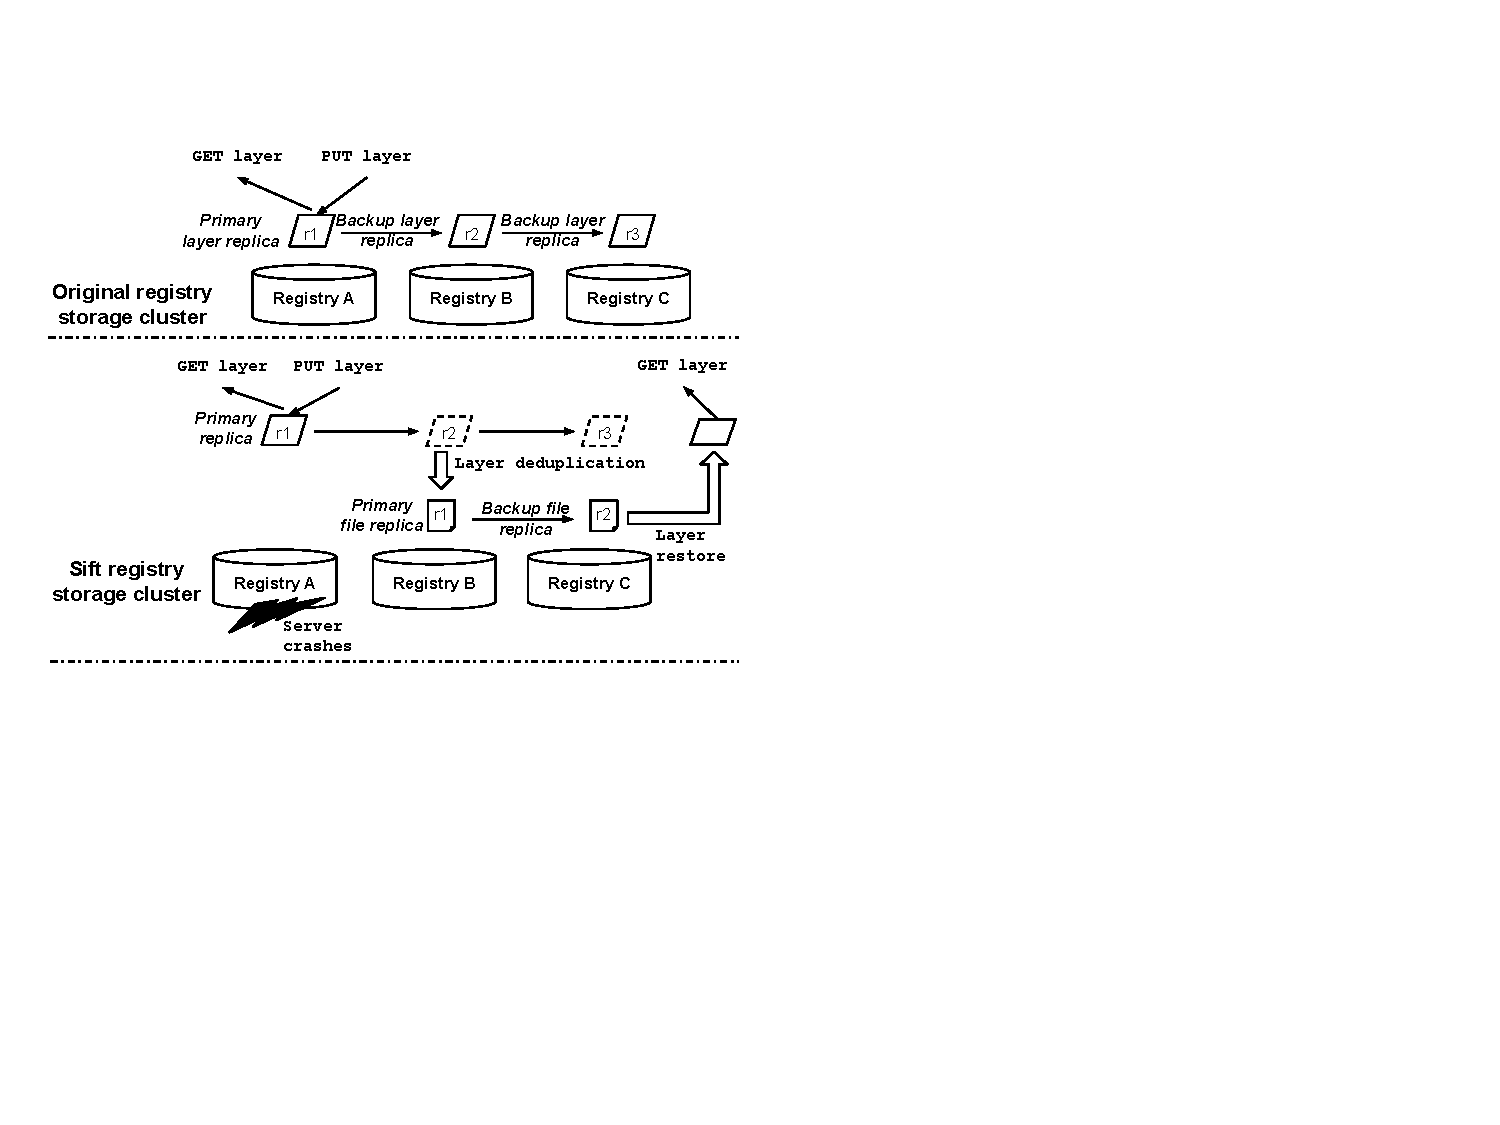
\includegraphics[width=0.35\textwidth]{graphs/sift-arch.pdf}
		\label{fig:sift-original}
	}
	\caption{Architecture of \sysname. \LR{The text in the figures is a bit too small. As a rule of thumb,
	text in figures should be as large as normal text.}}
	\label{fig:sys-overview}
\end{figure}